\documentclass[conference]{IEEEtran}
\usepackage{graphicx}
\usepackage{epstopdf}
\usepackage{array}
\usepackage{multirow}
\usepackage{multicol}
\usepackage{empheq}
\usepackage{algorithm}
\usepackage{algorithmicx}
\usepackage{algpseudocode}
\usepackage{amsmath}
\renewcommand{\algorithmicrequire}{ \textbf{Input:}} %Use Input in the format of Algorithm
\renewcommand{\algorithmicensure}{ \textbf{Output:}} %UseOutput in the format of Algorithm
% correct bad hyphenation here
\hyphenation{op-tical net-works semi-conduc-tor}
\begin{document}
\title{Parsing Tables from EDGAR with Python \\and Its Dockerization}
%
% author names and affiliations
\author{\IEEEauthorblockN{Jiali Cheng$^{1}$}
\IEEEauthorblockA{$^{1}$Graduate School of Engineering, Northeastern University, Boston, USA}
}
% make the title area
\maketitle
\begin{abstract}
We use Python to access data from EDGAR, the Electronic Data Gathering, Analysis, and Retrieval system. Given a company ID, called CIK, and an Access Number, called acc-no, an URL to this HTML file is generated. We locate to the 10Q file and extract all the tables and save them as CSV(Comma Separated Values) files. Then we dockerize this pipeline so that it can be used for any websites, not only restricted to IBM.
\end{abstract}
\begin{keywords}
Parse Tabels, HTML, EDGAR, Python, Docker
\end{keywords}
\IEEEpeerreviewmaketitle
%
%Introduction
\section{Introduction}\label{i}
\indent 
\begin{algorithm}\label{start}
\caption{Start, start running the whole process}
\begin{algorithmic}[1]
	\Ensure double k
	\Function {Master} {double curTime}
		\State $url \gets \Call {FormUrl}{acc-no}$
		\State $url\_10q \gets \Call {FormUrl}{acc-no}$
		\State $\Call {extract}{}$
	\EndFunction
\end{algorithmic}
\end{algorithm}
\indent The result of the parsed tables from the given URL is as follow:
\begin{figure*}
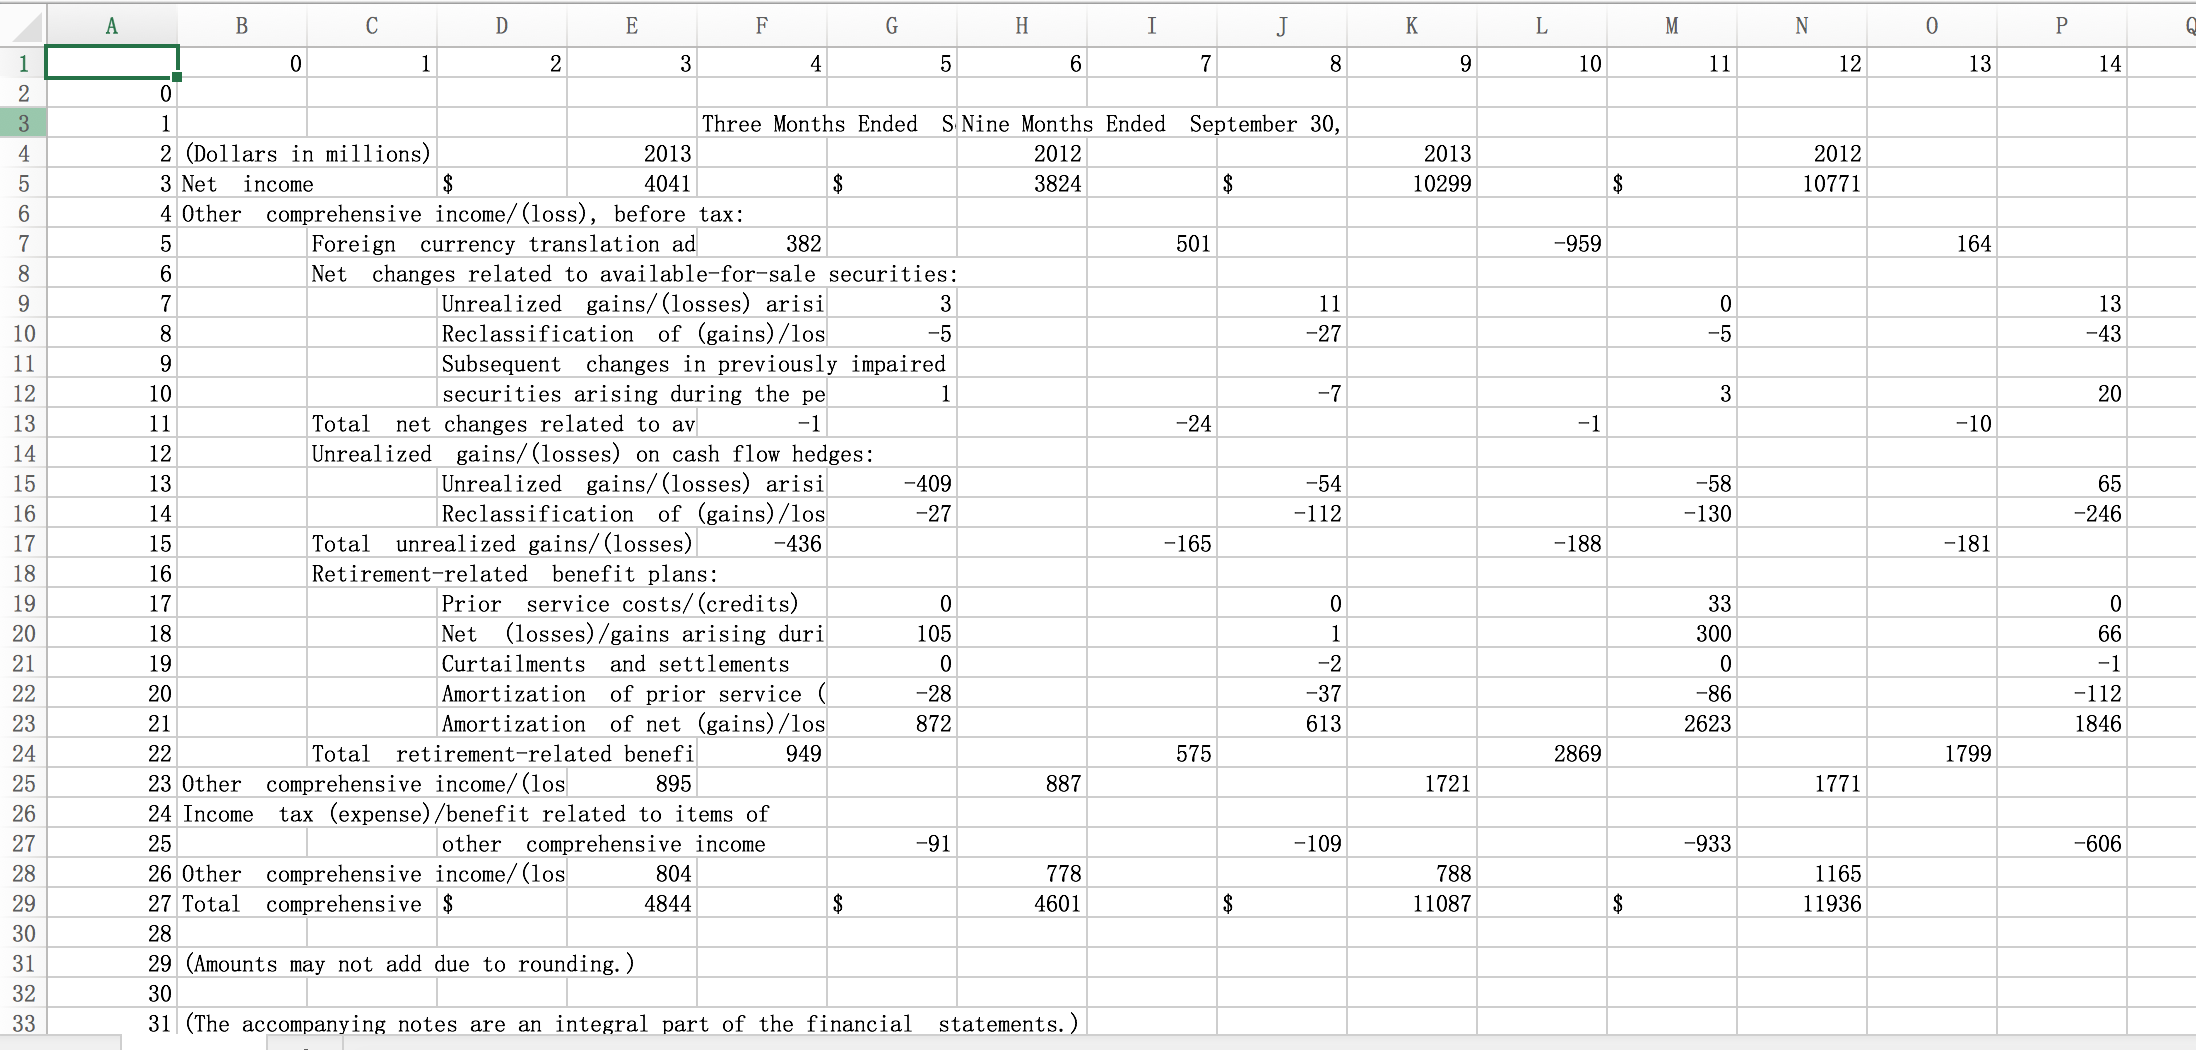
\includegraphics[width=6.0in]{table.png}
\caption{The flow diagram of the LCPR algorithm}\label{data}
\end{figure*}
%
\begin{algorithm}\label{extract}
\caption{Extract, extracting tables from the 10Q file}
\begin{algorithmic}[1]
	\Require url\_10q
	\Ensure double k			\Comment {Get an HTTP response according to the URL of 10Q file and transform the response into lxml form. Then find the HTML tags to get the table items.}
	\Function {Master} {double curTime}
		\State $response \gets \Call {Response}{url\_10q}$
		\State $soup \gets \Call {BeautifulSoup}{response}$
		\State $filename \gets acc-no$
		\State $\Call {Open\_CSV\_File}$
			\For $\Call {Find\_all}{'table'}$
				\For $\Call {Find\_all}{'th'}$
					\For $\Call {Find\_all}{'td'}$
						\State $\Call {Write\_Result}{filename}$
					\EndFor
				\EndFor
			\EndFor
	\EndFunction
\end{algorithmic}
\end{algorithm}
%
\section{Result}\label
\\
%
\section{Conclusion}\label{v}
\indent In this paper, we propose a way to parse tables in the 10Q file of a company in the EDGAR system. Then we dockerize this program to use it on other platforms. Results show that we have finish the job and reach the objectives.%
\begin{thebibliography}{1}
\bibitem{NASA's Space}
Liebrecht, P., Schier, J., Bhasin, K., Bibyk, I., Butler, M., Hudiburg, J., Tai, W., Shames, P., NASA's Space Communications Integrated Architecture, Proceedings of SpaceOps 2010 Conference, AIAA, 25-30 April 2010, Huntsville,
Alabama.
\end{thebibliography}
\end{document} 